\newpage


\section{Informationsarchitektur} \label{layout}

\subsection{Inhaltlicher Aufbau}

\begin{figure}[H]
    \caption{Seitenstruktur}
    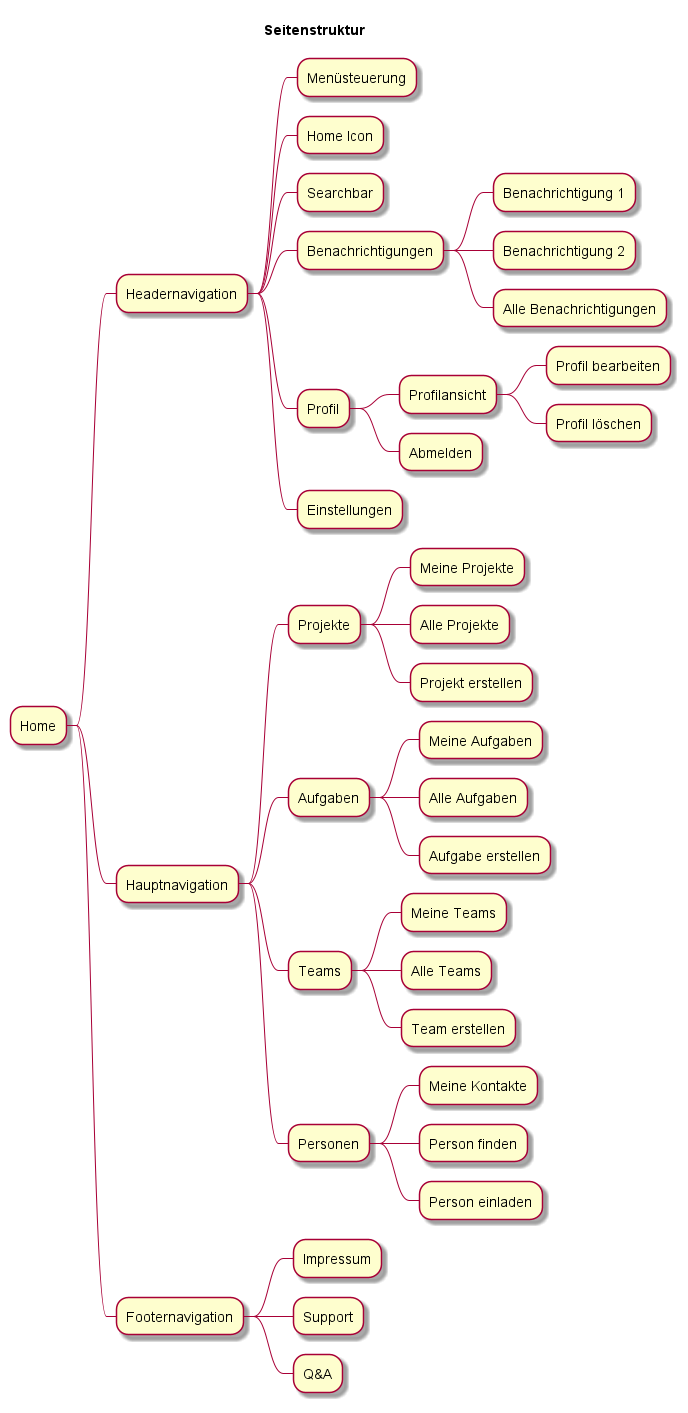
\includegraphics[width=0.9\textwidth,height=0.5\textheight]{plantuml/seitenstruktur}
    \\
    Quelle: Eigene Quelle
\end{figure}

Wie in der Abbildung Seitenstruktur dargestellt, orientiert sich die Seitenstruktur in drei grundlegende Bereiche.

\subsubsection{Betrieb}

Der Betrieb bildet die Fachlichkeit der \ac{SPA} ab.
Diese ist unterteilt in die vier Hauptobjekte, Projekt, Aufgaben, Teams und Personen.
Jedes dieser Objekte hat mögliche mit Ihm verbunde Operationen.
Um die Seitenstruktur möglichst flach und einheitlich zu halten, bietet jedes Hauptobjekt drei mögliche Unterkategorien.

\begin{description}
    \item[Meine <Objekte>] Die erste ist eine Selektierung der, falls vorhanden, sieben wichtigsten Objekte dieser Kategorie.
    Dies können zum Beispiel die sieben meistgenutzten Kontakte einer Person sein oder die aktuellsten Aufgaben.
    Diese werden je nach größe Tabellarisch oder als Karten angezeigt.
    Zusätzlich gibt es ein Element auf dieser Anzeige das zu einer vor gefilterten der nächsten Seite "Alle <Objekte>" leitet.
    \item[Alle <Objekte>] Unter diesem Punkt werden alle für den Nutzer sichtbaren Objekte einer Kategorie angezeigt.
    Diese Liste ist Filterbar und Pageable.
    Ebenfalls gibt es in solchen Listen, falls der Nutzer hierzu berechtigt ist, einen Button der zu dem Punkt "<Objekt> erstellen" führt.
    \item[<Objekt> erstellen] Unter diesem Punkt wird man zu einem Formular für die Anlage eines entsprechenden Objektes geleitet.
    Dieser Punkt ist nur sichtbar, wenn der Nutzer über eine entsprechende Berechtigung verfügt.
\end{description}

Alle dieser drei Seiten führen zu einer Instanz des Hauptobjektes.
Hier werden im Seiteninhalt neben der Objektansicht auch die restlichen Operationen und Unterobjekte des Objektes abgebildet.

\subsection{Seitenaufbau}

\subsubsection{Dashboard}

\begin{figure}[H]
    \caption{Seitenstruktur}
    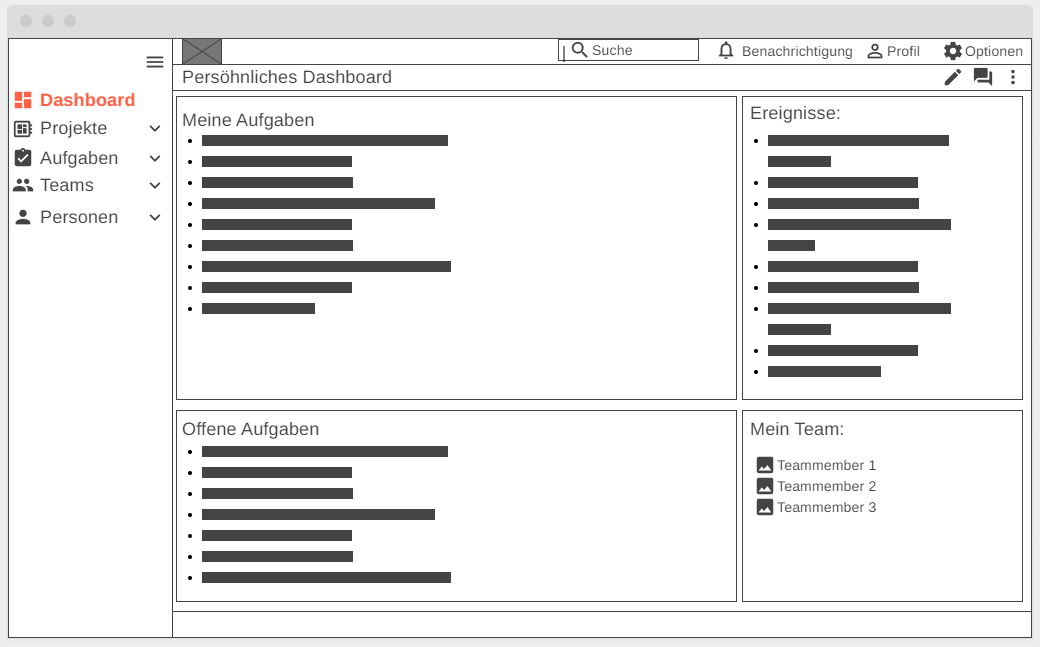
\includegraphics[width=0.9\textwidth]{wireframe/dashboard_qkQJUh}
    \\
    Quelle: Eigenes Wireframe: https://wireframe.cc/qkQJUh
\end{figure}

Die Startseite der Webseite ist entweder die Loginseite oder wenn bereits angemeldet das persönliche Dashboard des Nutzers.
Dieses ist Personalisierbar.
Es können maximal 7 Karten geladen werden.
Diese werden dynamisch angeordnet so, dass sie auf einen Bildschirm mit Breakpoint Large passen.
Bei kleineren Breakpoints erhält die Seite eine Scrollfunktion.

\subsubsection{Aufgabe}

\begin{figure}[H]
    \caption{Seitenstruktur}
    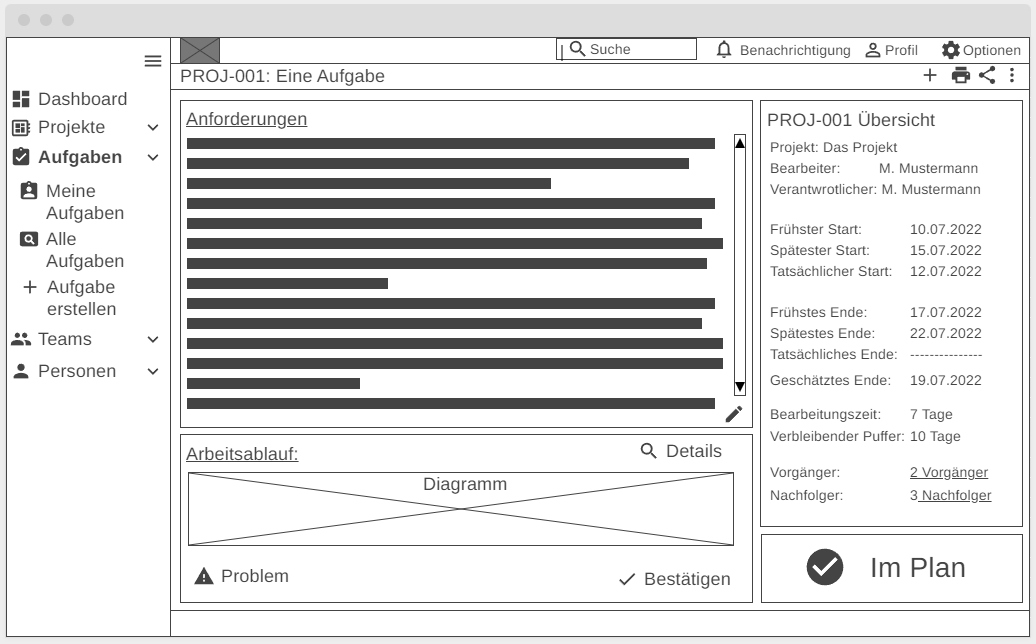
\includegraphics[width=0.9\textwidth]{wireframe/task_details_IyX8ei}
    \\
    Quelle: Eigenes Wireframe: https://wireframe.cc/IyX8ei
\end{figure}

Diese Seiten sind unter folgendem Kontextpfad erreichbar /app/aufgabe/proj-001.
Wobei proj-001 hier der Name bzw die ID der Aufgabe ist.
Von einer Aufgabe können folgende Seiten erreicht werden:

\begin{itemize}
    \item[/app/projekt/proj] Das Projekt der Aufgabe
    \item[/app/aufgabe/proj-001/historie] Die Historie der Aufgabe in tabellarischer Form
    \item[/app/aufgabe/proj-001/nachfolger] Die Nachfolger dieser Aufgabe als Kartenansicht
    \item[/app/aufgabe/proj-001/vorgaenger] Die Vorgänger dieser Aufgabe als Kartenansicht
    \item[/app/person/fgzjwhb] Die Profilseite des Autors oder des Bearbeiters
    \item[/app/projekt/proj/aufgabe/erstellen] Wenn Berechtigt, ein Formular zum erstellen einer neuen Projektaufgabe.
\end{itemize}

\subsection{Funktionaler Aufbau}

\subsubsection{Seitenlayout}

\begin{figure}[H]
    \caption{Seitenstruktur}
    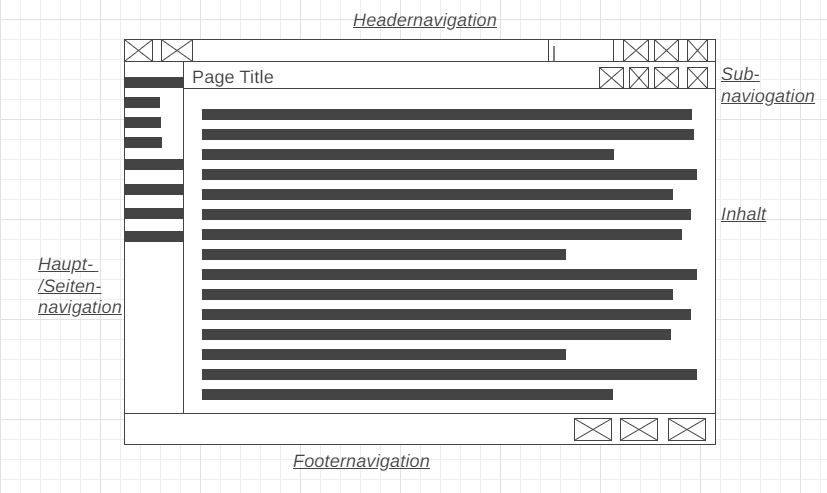
\includegraphics[width=0.9\textwidth]{wireframe/layout_bigger_middle}
    \\
    Quelle: Eigene Quelle
\end{figure}

Da die \ac{SPA} mehrere verschiedene Steuerelemente besitzt, werden diese in eigene fachliche Bereiche getrennt.
Hierbei entfällt die Programmsteuerung aus Abbildung 1 auf die Headernavigation.
Die Rubrik Betrieb wird in die Seitennavigation ausgelagert und Allgemeines landet in der Fußzeile.

Der Seiteninhalt ist abhängig von der aktuellen URL und hat eine eigene Subnavigation.
Diese kann Operationen in Form von Icon mit Tooltipp enthalten, die aktuell für die Seite Sinn machen.
Typisch hierfür wären, Teilen, Drucken, Hinzufügen und ähnliche auf den Inhalt bezogene Funktionen.
Diese Funktionen sind keine Hauptfunktionen und sollen somit auch um die Kopfzeile nicht überladen.
Dadurch entfällt ein beschreibender Text nur auf den Tooltipp.

\subsubsection{Responsivität}

Bei kleineren Endgeräten kann das vollständige Seitenlayout nicht beibehalten werden.
Hierzu wurden folgende Breakpoints definiert:

\begin{table}[H]
    \caption{Breakpoints}
    \label{tbl:breakpoints}
    \begin{tabularx}{\textwidth}[ht]{|l|l|}
        \hline
        \textbf{Breakpoint name} & \textbf{Media query} \\
        \hline
        XSmall                   & (max-width: 599.98px) \\
        Small                    & (min-width: 600px) and (max-width: 959.98px) \\
        Medium                   & (min-width: 960px) and (max-width: 1279.98px) \\
        Large                    & (min-width: 1280px) and (max-width: 1919.98px) \\
        XLarge                   & (min-width: 1920px) \\
    \end{tabularx}
\end{table}

Neben den Breakpoints enthält die nachfolgende Tabelle den Zustand, in dem sich Bestandteile des Grundlayouts befinden sollen, wenn die Bildschirmgröße im Breakpoint liegt.

\begin{table}[H]
    \caption{Verhaltenstabelle Responsives Layout}
    \label{tbl:verhaltRespons}
    \begin{tabularx}{\textwidth}[ht]{|l|l|X|}
        \hline
        \textbf{Komponente} & \textbf{Breakpoint}   & \textbf{Zustand}                                                                                \\
        \hline\hline
        Seitennavigation & XSmall, Small & Seitennavigation ist eine Mobile Advanced Hamburger Navigation, mit default Zustand geschlossen \\
        & Medium, Large, XLarge & Seitennavigation ist ein Collapsible-Menü, mit default Zustand offen                            \\
        \hline\hline
        Kopfzeile & XSmall, Small & Die Kopfzeile wird auf die Steuerung des Hamburgermenüs und dem Logo mit Seitennamen reduziert. Die anderen Steuerelemente werden in die Seitennavigation ausgelagert. \\
        & Medium & Die Kopfzeile wird um die vorher ausgelagerte Steuerungselemente Suchleiste, Benachrichtigungen, Profil und Einstellungen ergänzt. BEschreibungen der Steuerungen sind als Tooltipp verfügbar. \\
        & Large, XLarge & Tooltipps werden nun als Text zu den Steuerelementen hinzugefügt. \\
        \hline\hline
        Hauptinhalt & XSmall, Small & Ist bei offenem Seitenmenü im Hintergrund und nicht bedienbar \\
        & Medium, Large, XLarge & Passt sich an die Seitennavigation an und nimmt den rest des Bildschirms ein. Ist auch bei offenem Seitenmenü verwendbar. \\
        \hline\hline
        Zweite Kopfzeile & XSmall, Small, Medium & nicht verfügbar. FUnktionen sind nun nur in dem Bereich Einstellungen verfügbar. \\
        & Large, XLarge & Verfügbar und enthält aktuellen Seitentitel des angezeigten Inhaltes und dazugehörige Operationen wie Teilen oder Drucken \\
        \hline\hline
        Fußzeile & XSmall, Small & nicht verfügbar. Funktionen sind nun im unteren Bereich des Seitenmenüs als Links verfügbar\\
        & Medium, Large, XLarge & Verfügbar und enthält aktuellen Seitentitel des angezeigten Inhaltes und dazugehörige Operationen wie Teilen oder Drucken \\
        \hline
    \end{tabularx} \\
    \cite[Quelle: In Anlehnung an https://material.angular.io/cdk/layout/overview][S. 4]{Beckert.2012}
\end{table}

Die nachfolgende Grafik stellt exemplarisch das Pagelayout nach Breakpoint Small dar.

\begin{figure}[H]
    \caption{Seitenstruktur}
    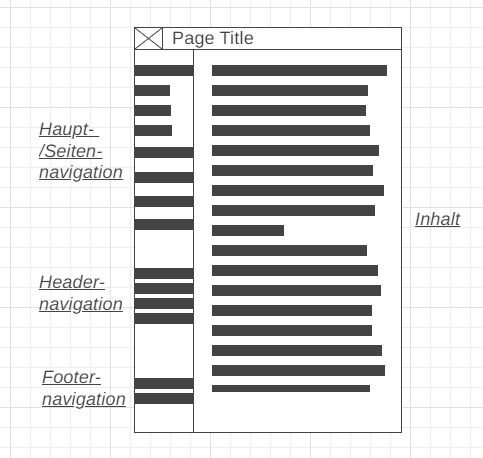
\includegraphics[width=0.9\textwidth]{wireframe/layout_small}
    \\
    Quelle: Eigene Quelle
\end{figure}

\subsubsection{}
